\section{Remote Vision Virtual Subsystem}%
\label{sec:remote-visi-subsyst-design}
The design specification devised in
Section~\ref{sec:remote-visi-subsyst-design} can now be implemented to the
target platform to fulfill the remote vision and telemetry functionalities
required. In this section the relevant implementation details are
addressed on the hardware and software domains.
%
\subsection{Hardware}%
\label{sec:hardware-rvvs-implem}
In the design stage, and in the first iterations of the
implementation, it is perfectly reasonable to adopt general domain environments,
such as virtual machines. Nonetheless, one must keep in mind that, ultimately,
the devised software will be running on hardware nodes. Thus, an important implementation step is the selection of the target
platform, taking into considerion several design criteria, such as, throughput,
memory footprint, storage, response time, connectivity, etc.

An example of a viable platform is the Raspberry Pi Zero W (Fig.~\ref{fig:pi-zero-w}), which is a low cost
board design (it retails for about 5 EUR) around the Broadcom system on-chip (SoC) BCM2835, which includes a
1 GHz single-core ARMv6 CPU, with a 64-bit architecture, allowing it to run
the full range of GNU/Linux distribution. Among other resources, it includes 512
MB RAM, VideoCore IV GPU, 40 GPIO pins, mini HDMI and micro-USB ports,
\gls{csi} connector, Micro SD Card Slot and on-board Bluetooth Low Energy (BLE)
4.1 and Wi-Fi based.

The Raspberry Pi Zero W provides the required communications
(Bluetooth and Wi-Fi) and camera interfaces, on a fully-fledged environment
capable of running 64-bit OS and at low cost, thus, making it
suitable for the implementation. Additionally, it packs in a small form-factor,
even with the inclusion of the camera, as illustrated in
Fig.~\ref{fig:pi-zero-w-cam}. The camera module has several models ranging from
5 to 12 megapixel resolution with high quality video capture (up to 1080p30) in
the 20--35 EUR pricepoint.
%
% Pi Zero W
\begin{figure}[!hbt]
\centering
    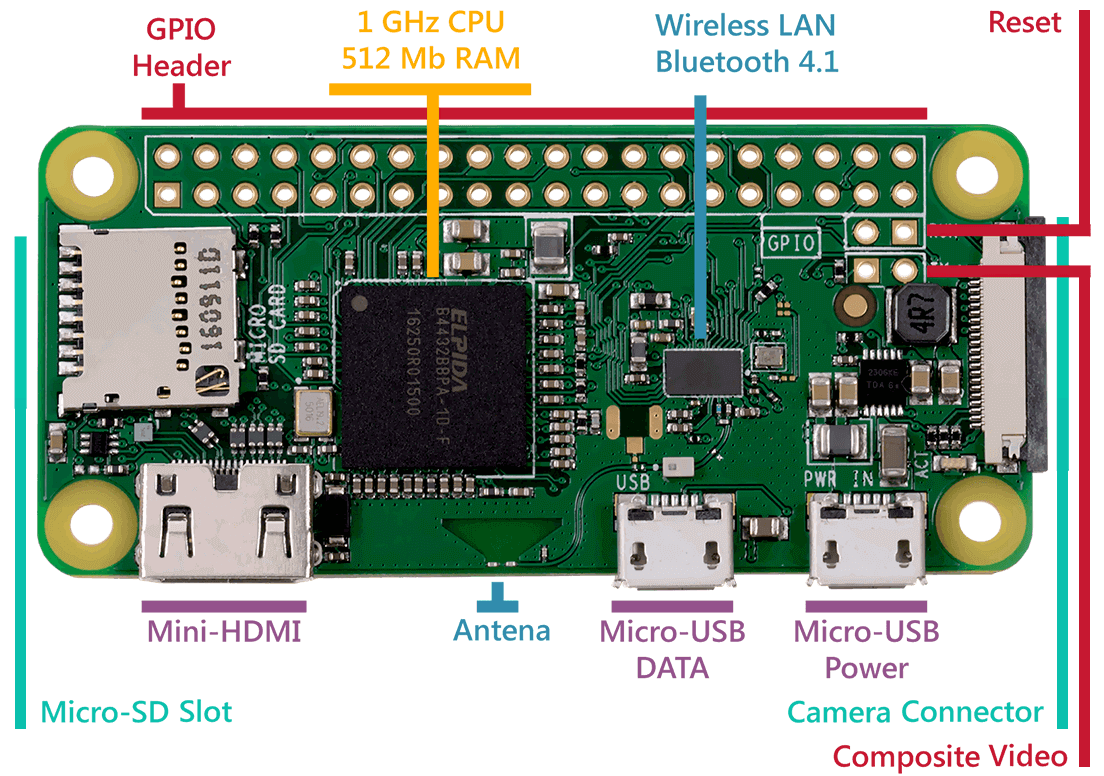
\includegraphics[width=0.6\textwidth]{./img/pi-zero-w.png}
  \caption{Raspberry Pi Zero Wireless overview}%
\label{fig:pi-zero-w}
\end{figure}
% Pi Zero W Camera
\begin{figure}[!hbt]
\centering
    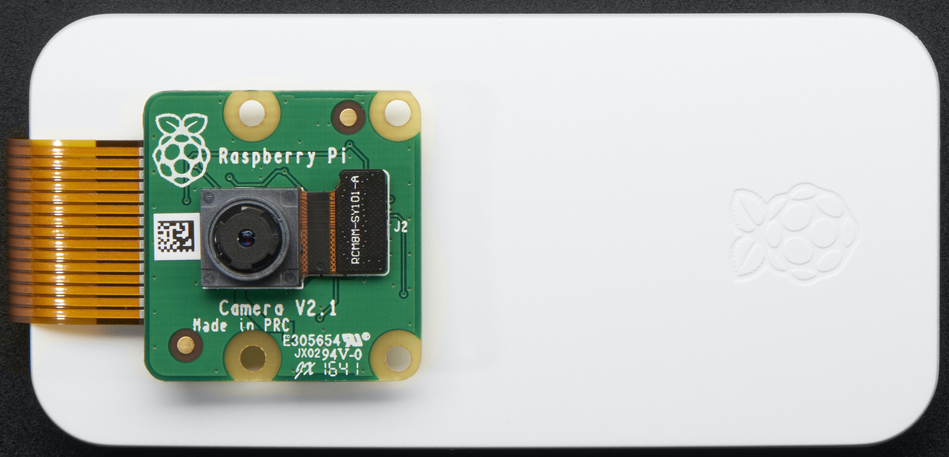
\includegraphics[width=0.6\textwidth]{./img/pi-zero-w-cam.jpg}
  \caption{Raspberry Pi Zero Wireless overview}%
\label{fig:pi-zero-w-cam}
\end{figure}
%
%
\subsection{Software}%
\label{sec:software-rvvs-implem}
The software part is mainly comprised of two main components: the software
environment support and the actual software running on top of that. The software
environment provides the low-level layer(s) that interfaces the hardware,
typically under some form of an \gls{os} and the associated development
toolchain required to target the platform.

In the present case, the selected platform --- Raspberry Pi --- supports
64-bit GNU/Linux based operating systems, which can be used to bootstrap the
implementation. Nonetheless, it is desirable to maintain the code footprint and
dependencies as low as possible, as required in the majority of the embedded
systems, thus, a custom tailored Linux OS can be used. Contemplating the build
tools required for the deployment of a tailored Linux OS, there are several
solutions, such as, Buildroot, Yocto and OpenWRT. The selected build tool was
Yocto, an open-source project project that provides templates, tools, and
methods to help you create custom Linux-based systems for embedded products
regardless of the hardware architecture~\cite{yocto2020}. Additionally, it is
required the cross-compilation toolchain that enables deployment to target from
host. Yet, in this initial implementation phase, the \gls{rvvs} susbsystem is
virtualized in a Linux \gls{vm}, thus, sparing this step for now. However, after
implementing and testing the application in the Linux \gls{vm}, this approach
should be relatively straightforward, enabling fast deployment to the real
hardware.

Hence, in the following sections, it is discussed the implementation of the
\gls{rvvs} stack designed in Section~\ref{sec:subsyst-decomposition-rvvs}.
%
\subsubsection{Image Acquisition}%
\label{sec:img-acq-rvvs-implem}
The usage of the Linux \gls{vm} has another inherent advantage, associated to
the UNIX philosophy in which it is based, that everything is a file (except for
the network part). As a matter of fact, every device attached to the Linux OS
can be easily and transparently accessed, e.g., via the \texttt{/dev}
directory. Additionally, as every device is a file, the file \gls{api} can be
used to manage the device, using the typical system calls \texttt{open/close}
and \texttt{read/write}.  

The typical call stack for image acquisition and streaming is comprised of:
low-level drivers that interface the hardware via the kernel (dependent on the
type of interface), dealing with frame capture (e.g., \gls{v4l}); and the
commonly named \emph{frame grabber}, which takes the raw frames and encodes it
into streams, for posterior multiplexing into their final container (e.g.,
\texttt{ffmpeg}).

The \gls{v4l2} is the second version of the \gls{api} and framework, which is an
integral part of the Linux kernel code, as opposed to many driver
implementations~\cite{v4l2-headers}. The \gls{v4l2} \gls{api} is mostly
implemented as set of \texttt{ioctl} (control device) system
calls~\cite{kerrisk2010linux} that enable easy manipulation of video devices.
\emph{The workflow for a typical \gls{v4l2} application is as follows}:
\begin{enumerate}
\item Open a descriptor to the device;
\item Retrieve and analyse the device's capabilities. V4L2 allows you to query a
  device for its capabilities, that is, the set of operations (roughly, IOCTL
  calls) it supports;
\item Set the capture format: frame size, format (MJPEG, RGB, YUV, \ldots),
  etc.; check the device handles the format.
\item Prepare the device for buffer handling. When capturing a frame, it has
  to submitted a buffer to the device (\texttt{queue}), and retrieved it once
  it's been illed with data (\texttt{dequeue}). However, before this, the device
  must be informed about the buffers (buffer request).
\item For each buffer, certain aspects must be negotiated with
  the device (buffer size, frame start offset in memory), and then created a new
  memory mapping for it.
\item Put the device into streaming mode.
\item Once the buffers are ready, it is only required the queueing/dequeuing
  of the buffers repeatedly, and every call will grab a new frame. The delay
  defined between each frames by putting the program to sleep is what
  determines the framerate.
\item Turn off streaming mode.
\item Close your descriptor to the device.
\end{enumerate}

The \gls{v4l2} \gls{api} is implemented in the \texttt{C} programming
language. Thus, a basic wrapper class was implemented in \texttt{C++} to
abstract from the low-level details and increase modularity, following the
aforementioned workflow.

Listing~\ref{lst:webcam-h} provides the webcam interface (public and private)
using the V4L2 API. The construtor takes the type of capture to perform, e.g.,
video capture, and the associated memory type. The open/close member functions
enable the opening and closing of the file descriptior associated with the
device. \texttt{setFormat} sets the image format and dimensions,
\texttt{startStream} starts the stream and writes the output to a file, and
\texttt{setRequestBuffer} defines the number of buffers to use. In the private
interface lies the \texttt{allocateBuffer} and \texttt{open} member functions which allocates a
buffer for the device on behalf of the \texttt{setRequestBuffer}. As private
variables there are the file descriptor associated with the device
\texttt{m\_FileDescriptor}, the pointer to a buffer frame \texttt{m\_bufferPtr},
and the V4L2 variables representing the buffer's type, memory type and
capabilities, respectively. Additionally, a mutually exclusive object variable
\texttt{m\_mutex} is used to manage concurrent access to the device via file descriptor.\\
% Webcam header file
\lstinputlisting[language=C++, caption={Webcam wrapper interface using the V4L2 API},label=lst:webcam-h,
style=customc]{./listing/webcam-v4l2.h}%

Next, a small driver program (Listing~\ref{lst:webcam-main}) was devised to test
the webcam interface. The device location is set to \texttt{/dev/video0} where
the attached camera is placed under Linux filesystem. A webcam object is created
for video capture and then is tried out the aforementioned workflow by opening
the device, setting the dimensions to 320x240 pixels and the format to Motion
JPEG (MJPEG), requesting one buffer, starting the stream to an output file and
finally closing the device.\\ 
% Webcam main
\lstinputlisting[language=C++, caption={Webcam driver program},label=lst:webcam-main,
style=customc]{./listing/webcam-main.cpp}%

Later on, the client code that uses the Webcam interface was added to
respective thread, responsible for starting a webcam stream on user-demand.
%
\subsubsection{Wi-Fi}%
\label{sec:wi-fi-rvvs-implem}
For the implementation of the Wi-Fi communication, \gls{tcpip} sockets were used
in conjunction with the client/server architecture. Although only the server is
running on the \gls{rvvs} subsystem, the instantiation of both client and server
enables the testing of the complete communications workflow, without the need to
add the uncertainty associated with the communication medium.


%  UTILITY FUNCTIONS:
%  One must specially careful with the byte ordering (aka endianess), so one does not get
%  "translations" mistakes. In that sense, one must remember two things:
%  	1. The network byte ordering is always big endian.
%  	2. Before sending data packets to the network, one must always convert it to 
%          network byte ordering.
%  For this purpose, we use the following utility functions:
%  + Byte Ordering:
%   - Host Byte Order to Network Byte Order:
%   	- short: htons();
%   	- long:  htonl().
%   - Network Byte Order to Host Byte Order:
%   	- short: ntohs();
%   	- long:  ntohl();
%
%  + IP Adress format:
%   - ASCII dotted to Binary: inet_aton()
%   - Binary to ASCII dotted: inet_ntoa()
%  
%  + Padding
%   - bzero: write zeroes to a byte string
%   	bzero(void *s, size_t n);

%
%%% Local Variables:
%%% mode: latex
%%% TeX-master: "../../../dissertation"
%%% End:
